\documentclass[aspectratio=1610]{beamer}

\usepackage{./util/zariski}

\usepackage{csquotes}
\usepackage{tikz}

\usetheme{Hannover}
% \usecolortheme{crane}
\setbeamertemplate{navigation symbols}{}

\author{Matthias Hutzler}
\title[Synthetic Algebraic Geometry]{Introduction to\\Synthetic Algebraic Geometry}
\date{Proof and Computation 2023\\Herrsching}


\begin{document}

\begin{frame}
  \maketitle
\end{frame}

\section{Overview}

\begin{frame}
  \frametitle{What is synthetic algebraic geometry?}

  \begin{description}[synthetic algebraic geometry]
    \item[algebraic geometry]
      Thinking about algebra in geometric terms.
    \item[synthetic algebraic geometry]
      Thinking about algebra in geometric terms,\\
      using a \alert{special language} that makes complex constructions look simple.
  \end{description}
  \bigskip
  \pause%
  \begin{itemize}
    \item
      language: homotopy type theory (HoTT) + special axioms
    \item
      model: Zariski $\infty$-topos
  \end{itemize}
\end{frame}

\begin{frame}
  \frametitle{What is synthetic algebraic geometry?}

  \center%
  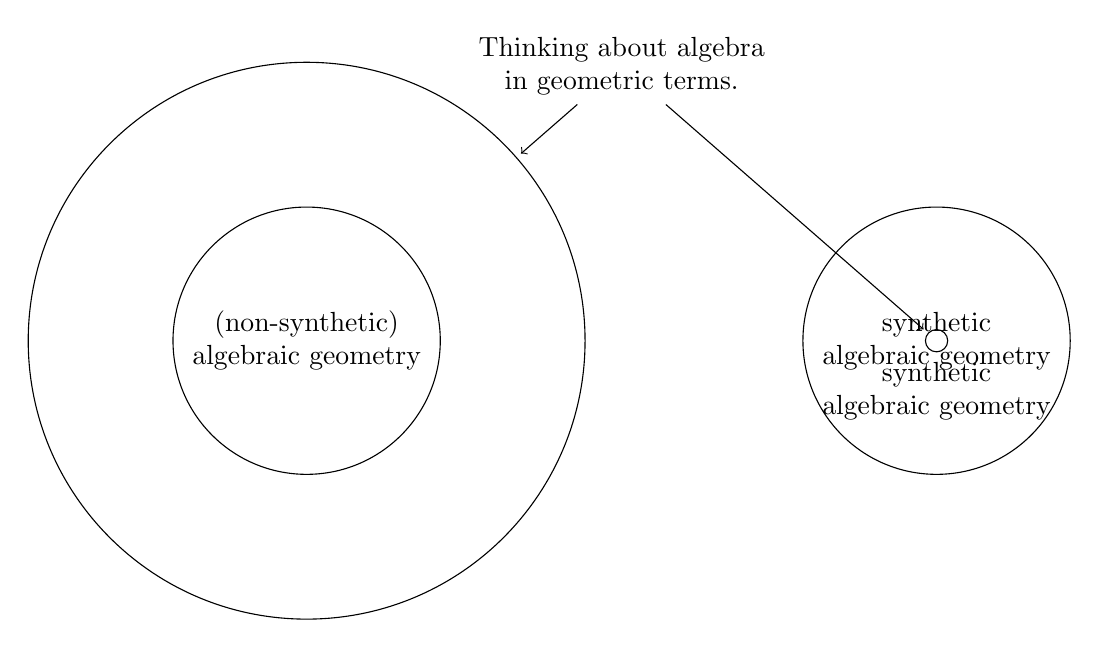
\begin{tikzpicture}
    % need align=* for line breaks
    \node[above,align=center] at (0,0) (start) {Thinking about algebra\\in geometric terms.};

    \node<1>[circle,draw,inner sep=1.2cm] at (-4,-3) (left) {};
    \node<2>[circle,draw,inner sep=2.5cm] at (-4,-3) (left) {};
    \node[align=center] at (left) {(non-synthetic)\\algebraic geometry};
    \node<1>[circle,draw,inner sep=1.2cm] at (4,-3) (right) {};
    \node<2>[circle,draw,inner sep=0.1cm] at (4,-3) (right) {};
    \node<1>[align=center] at (right) {synthetic\\algebraic geometry};
    \path<2> (right.south) node[below,align=center]{synthetic\\algebraic geometry};

    \draw[->,shorten >=2pt] (start) -- (left);
    \draw[->,shorten >=2pt] (start) -- (right);
  \end{tikzpicture}
\end{frame}

\begin{frame}
  \frametitle{Current work (since 2022)}

  \begin{block}{Preprint}
    F. Cherubini, T. Coquand, M. Hutzler,
    \textit{A Foundation for Synthetic Algebraic Geometry}\\
    \url{https://arxiv.org/abs/2307.00073}
  \end{block}

  \begin{block}{People involved}
    Peter Arndt,
    Ingo Blechschmidt,
    Felix Cherubini,
    Thierry Coquand,
    Matthias Hutzler,
    Hugo Moeneclaey,
    David Jaz Myers,
    Marc Nieper-Wißkirchen,
    David Wärn,
    \dots
  \end{block}

  \begin{block}{Next workshop}
    2023-10-02 -- 2023-10-06, Augsburg\\
    \url{https://felix-cherubini.de/sag-meeting-3.html}
  \end{block}
\end{frame}

\begin{frame}
  \frametitle{Why \alert{you} might be interested}

  \begin{itemize}
    \item
      apply constructive reasoning
    \item
      apply homotopy type theory
    \item
      understand some algebraic geometry
  \end{itemize}
\end{frame}

\section{The spectrum of an algebra}

\begin{frame}
  \frametitle{Review of basic abstract algebra}

  \emph{ring}?
  \emph{algebra}?

  An $R$-algebra $A$ is \emph{finitely presented} if
  \[ A = R[X_1, \dots, X_n]/(p_1, \dots, p_m) \rlap{.}\]
\end{frame}

\begin{frame}
  \frametitle{$\Spec(A)$ does not faithfully represent $A$}
  $X^2 = 0$
\end{frame}

\begin{frame}
  \frametitle{Understanding algebraic subtleties geometrically}

  How is $X = 0$ different from $X^2 = 0$ geometrically?
  \bigskip

  \begin{columns}<2->
    \begin{column}{.5\textwidth}
      \[\begin{cases}
        X = 0 \\
        Y = 0
      \end{cases}\]
      \center%
      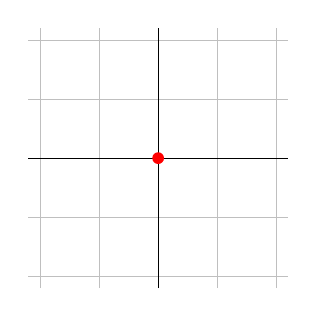
\begin{tikzpicture}[scale=1.5,domain=-1.1:1.1]
        \draw[very thin,color=lightgray,step=0.5] (-1.1,-1.1) grid (1.1,1.1);
        \draw plot (0,\x);
        \draw plot (\x,0);
        \path<3-> (0,0) node[red,circle,fill,inner sep=1.5pt]{};
      \end{tikzpicture}
      \center%
      \uncover<3->{a point}
    \end{column}
    \begin{column}{.5\textwidth}
      \[\begin{cases}
        X^2 - Y = 0 \\
        Y = 0
      \end{cases}\]
      \center%
      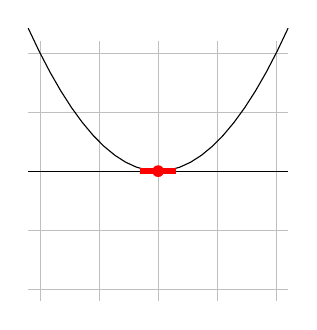
\begin{tikzpicture}[scale=1.5,domain=-1.1:1.1]
        \draw[very thin,color=lightgray,step=0.5] (-1.1,-1.1) grid (1.1,1.1);
        \draw plot (\x,\x*\x);
        \draw plot (\x,0);
        \path<3-> (0,0) node[red,circle,fill,inner sep=1.5pt]{};
        \draw<3->[red,line width=2pt] (-0.15,0) -- (0.15,0);
      \end{tikzpicture}
      \center%
      \uncover<3->{an \enquote{infinitesimally thickened} point}
    \end{column}
  \end{columns}
\end{frame}

\section{The axiom SQC}

\begin{frame}
  \frametitle{The axiom SQC}
\end{frame}

\begin{frame}
  \frametitle{Motivation for non-affine schemes}

  \begin{example}
    The two equations

    are equivalent:
  \end{example}

  We want to consider the space of all \alert{ratios} $[x : y : z]$
  for $x, y, z : R$.
\end{frame}

\begin{frame}
  \frametitle{Line bundles}
\end{frame}

\begin{frame}
  \frametitle{
\includegraphics[width=5cm]{./images/agda-logo.png}}

  Agda is
  \begin{itemize}
    \item
      a functional programming language
      \begin{itemize}
        \item
          influenced by Haskell
      \end{itemize}
    \item
      a proof assistant
      \begin{itemize}
        \item
          with a \alert{cubical type theory} mode
      \end{itemize}
  \end{itemize}
\end{frame}

\end{document}
